%% Figura do fluxo de data airlock (capitulo 3). Fonte da figuras/airlock.pdf.
%% Compile com:  cd figuras && pdflatex airlock.tex
\documentclass[tikz,border=2pt]{standalone}
\usepackage[T1]{fontenc}
\usepackage[utf8]{inputenc}
\usepackage{mathptmx}
\usetikzlibrary{positioning,arrows.meta}
\begin{document}
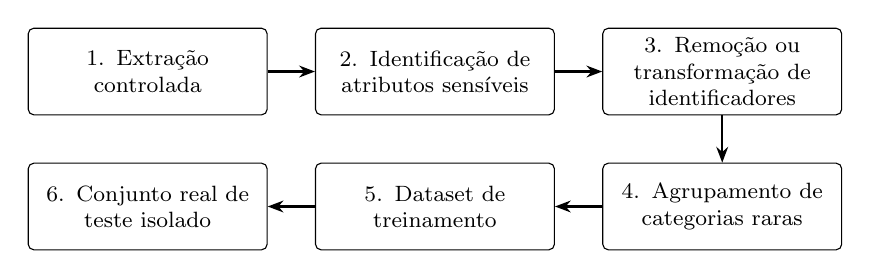
\begin{tikzpicture}[
    etapa/.style={draw, rounded corners=2pt, align=center, font=\footnotesize,
                  minimum width=30mm, minimum height=11mm, text width=28mm},
    seta/.style={-{Stealth[length=2mm]}, thick},
    node distance=6mm and 6mm]
  \node[etapa] (e1) {1. Extração\\controlada};
  \node[etapa, right=of e1] (e2) {2. Identificação de\\atributos sensíveis};
  \node[etapa, right=of e2] (e3) {3. Remoção ou\\transformação de\\identificadores};
  \node[etapa, below=of e3] (e4) {4. Agrupamento de\\categorias raras};
  \node[etapa, left=of e4] (e5) {5. Dataset de\\treinamento};
  \node[etapa, left=of e5] (e6) {6. Conjunto real de\\teste isolado};
  \draw[seta] (e1) -- (e2);
  \draw[seta] (e2) -- (e3);
  \draw[seta] (e3) -- (e4);
  \draw[seta] (e4) -- (e5);
  \draw[seta] (e5) -- (e6);
\end{tikzpicture}
\end{document}
